\section{Databricks vs. EMR Presto reference results}\label{referenceResults}

This section presents the reference results obtained by executing the full TPC-DS benchmark at the 1 TB scale factor employing the hardware and software configuration described in Section \ref{experimentalSetup}.

\subsection{Data loading}\label{referenceResultsDataLoading}

The TPC-DS Toolkit includes a data generator that produces raw text files that can be subsequently processed by a data framework to generate data files and accompanying metadata suitable for efficient query processing. The metadata is stored in a Hive-compatible metastore and the data in column-storage format files.

The raw text files generated for the 1 TB scale factor chosen for the reference results actually add up to 910.7 GB. The files were generated with 4 parallel streams, thus for some tables the data comprises 4 separate files, which are stored in the same directory. The format is raw text with the octal character \textbackslash 001 used as the column separator, which is the default in both Databricks and EMR Presto. It should be noted, however, that (unlike Databricks) EMR Presto does not allow in its supported syntax to employ an alternative character as separator. All of these files are stored in their respective directories within a common AWS S3 bucket.

The raw text files are used to create external tables by means of custom CREATE TABLE statements for Databricks and EMR Presto. We use these tables only for accessing data, not query processing. Additional CREATE TABLE statements are used to create another set of external tables employing a column-storage format, these meant for query processing. The data from the raw text external tables is fed to the external column-storage tables by means of INSERT INTO statements. The column-storage table files are also stored in S3. The format used for Databricks is Parquet with SNAPPY compression; the files add up to 297.5 GB, yielding a compression ratio of 3.26. Although Presto also supports the Parquet format, experiments showed that better results are achieved with the ORC format, using SNAPPY compression as well. The ORC files for Presto add up to 246.1 GB, resulting in a compression ratio of 3.94.

It is important to remark that for the reference results we present in this section, the tables were not explicitly analyzed to yield table and column statistics for optimization. The generation of table-level or basic statistics is different for each system. EMR Presto generates them by default with the execution of the INSERT INTO statements, which does not occur with Databricks. Thus for the query processing experiments, unless stated otherwise, EMR Presto has basic table statistics available while Databricks does not. In addition, neither system produces by default column-level statistics. Although Presto has the capability to compute column statistics, our EMR Presto configuration employs AWS Glue for table metadata, which does not support column statistics. On the other hand, Databricks does support them and we explore their effects in Section \ref{databricksWithStatistics}. Finally, we remark that we did not consider custom data partitioning in any of our experiments.

The behavior of the systems in regards to the data loading process as described above is summarized in Figure 18.

\begin{figure}
   \begin{center}
   \scalebox{0.65}{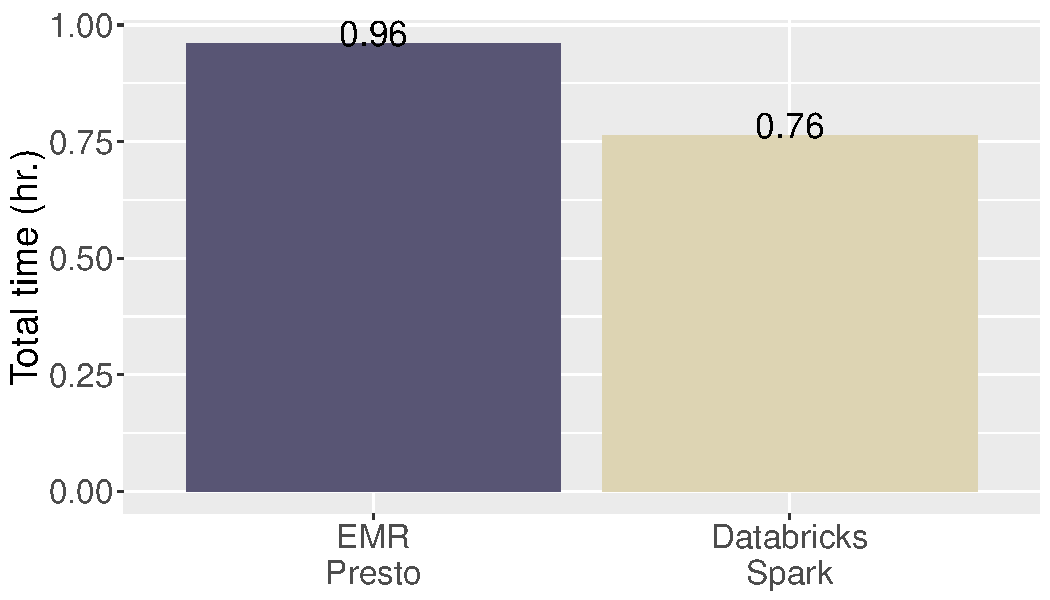
\includegraphics[width=7.0in]{imgs/referenceResults/load_totalHrTimeBarChart.pdf}}
   \end{center}
   \caption{Reference results Data Loading Test total time.}
   \label{fig:referenceResultsDataLoading}
\end{figure}

\subsection{Individual query execution (Power Test)}\label{referenceResultsPowerTest}

The data loading process takes about one hour on EMR Presto, whereas on Databricks it takes around 45 minutes. Although the difference is not major, it is significant. We also point out that Presto generates one file for each worker node, thus 8 files are generated in our setup. On the other hand, Databricks generates one file for each task, yielding over 300 files for some tables. Additional experiments would be required to determine if consolidating the files would result in performance improvements.

The TPC-DS schema includes 7 fact tables, one for the product inventory and 2 for each sales channel sales and returns, the channels being stores, catalog, and the web. A total of 17 dimension tables complete the schema. The fact tables have by far the largest data size, which we can confirm by looking at the individual table creation times, shown in Figure \ref{fig:referenceResultsDataLoadingIndTimes1} and Figure \ref{fig:referenceResultsDataLoadingIndTimes2}. The corresponding table names are given in Table \ref{table:tpcdsTableNames}. We note that the dbgen\_version table was not created since it is not used in queries and it employs data types with no direct equivalent in the SUTs.

\begin{table}
  \centering
	\begin{tabular}{|l|l|l|}
	  \hline
		\makecell[l]{1) call\_center \\
		2) catalog\_page \\
		3) catalog\_returns \\
		4) catalog\_sales \\
		5) customer \\
		6) customer\_address \\
		7) customer\_demographics \\
		8) date\_dim}
		&
		\makecell[l]{
		9) dbgen\_version (skipped) \\
		10) household\_demographics \\
		11) income\_band \\
		12) inventory \\
		13) item \\
		14) promotion \\
		15) reason \\
		16) ship\_mode}
		& 
		\makecell[l]{
		17) store \\
		18) store\_returns \\
		19) store\_sales \\
		20) time\_dim \\
		21) warehouse \\
		22) web\_page \\
		23) web\_returns \\
		24) web\_sales \\
		25) web\_site}
		\\ 
		\hline
	\end{tabular}
	\caption{TPC-DS table names.}
	\label{table:tpcdsTableNames}
\end{table}

\begin{figure}
   \begin{center}
   \scalebox{0.65}{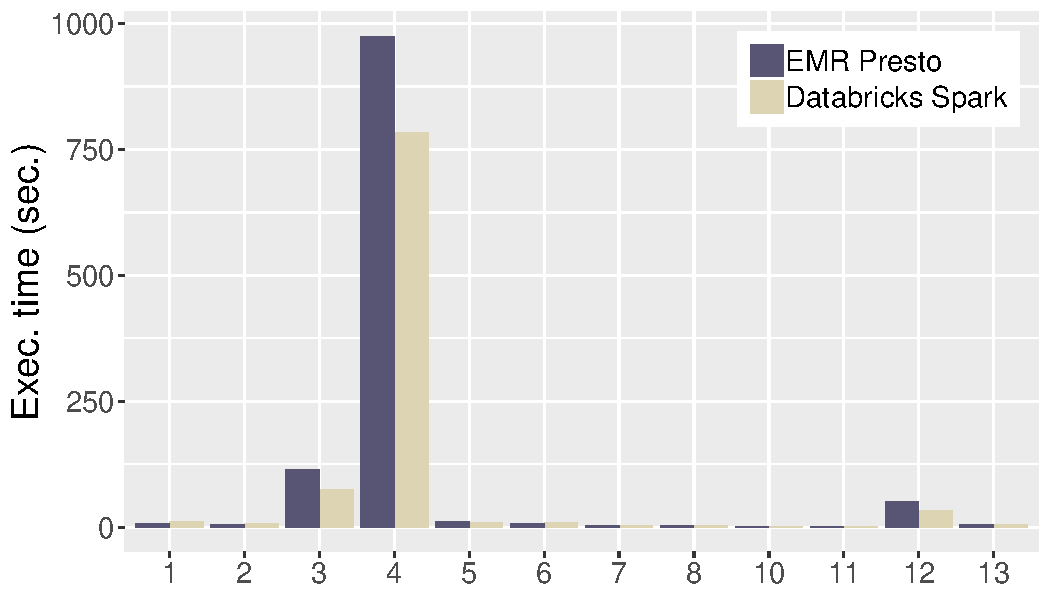
\includegraphics[width=7.0in]{imgs/referenceResults/loadTestIndivTables1.pdf}}
   \end{center}
   \caption{Reference results Data Loading Test individual table loading times (1).}
   \label{fig:referenceResultsDataLoadingIndTimes1}
\end{figure}

\begin{figure}
   \begin{center}
   \scalebox{0.65}{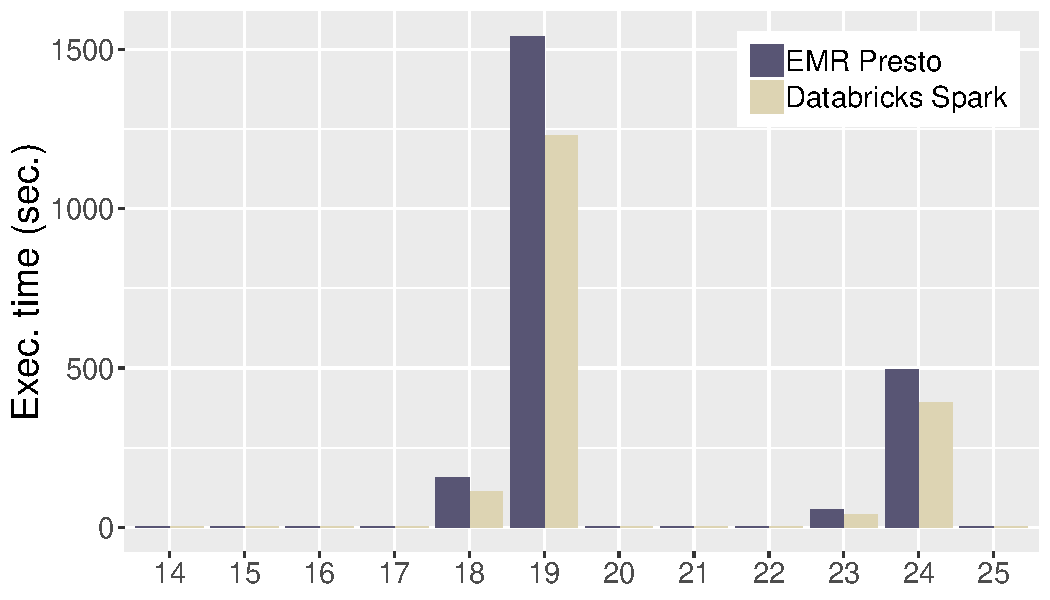
\includegraphics[width=7.0in]{imgs/referenceResults/loadTestIndivTables2.pdf}}
   \end{center}
   \caption{Reference results Data Loading Test individual table loading times (2).}
   \label{fig:referenceResultsDataLoadingIndTimes2}
\end{figure}

Clearly, the table creation times for the fact tables are proportional in all cases to the total database creation time. Furthermore, the creation time of the dimension tables is negligible.

\subsection{Individual query execution (Power Test)}

Next, we present the reference results for the TPC-DS Power Test, which implies running the 99 benchmark queries sequentially. We use the configuration stated in Section 3 and the 1 TB dataset created as described above. Figure \ref{fig:referenceResultsPowerTestTotalTime} gives the total time for both systems, while Figure \ref{fig:referenceResultsPowerTestGeomean} and Figure \ref{fig:referenceResultsPowerTestArithmeticMean} present the query execution time geometric mean and the query execution time arithmetic mean, respectively.

\begin{figure}
   \begin{center}
   \scalebox{0.65}{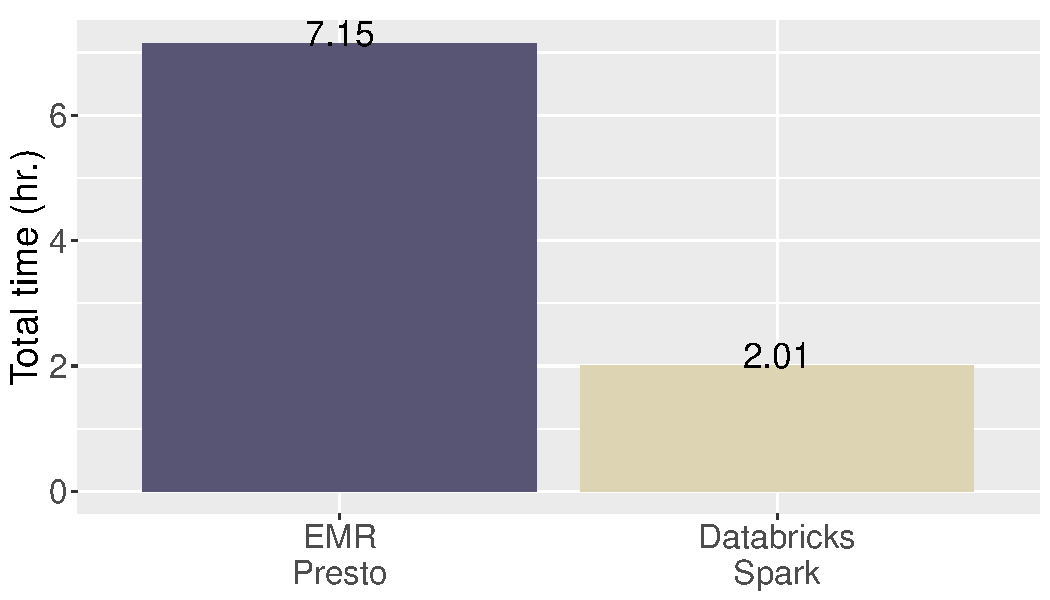
\includegraphics[width=7.0in]{imgs/referenceResults/power_totalHrTimeBarChart.pdf}}
   \end{center}
   \caption{Reference results Power Test total time.}
   \label{fig:referenceResultsPowerTestTotalTime}
\end{figure}

\begin{figure}
   \begin{center}
   \scalebox{0.65}{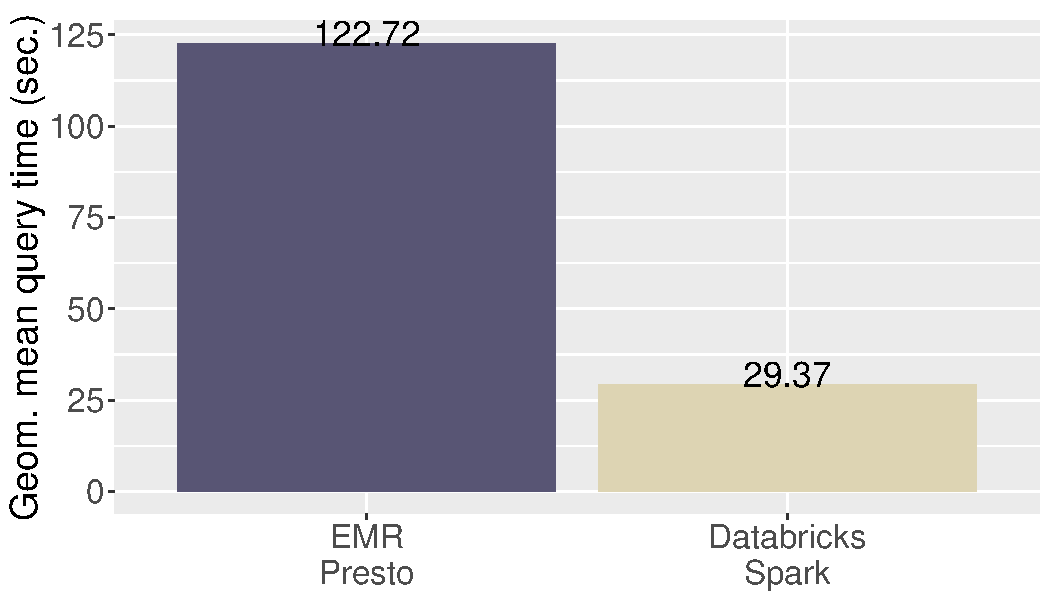
\includegraphics[width=7.0in]{imgs/referenceResults/power_geomeanTimeBarChart.pdf}}
   \end{center}
   \caption{Reference results Power Test query execution time geometric mean.}
   \label{fig:referenceResultsPowerTestGeomean}
\end{figure}

\begin{figure}
   \begin{center}
   \scalebox{0.65}{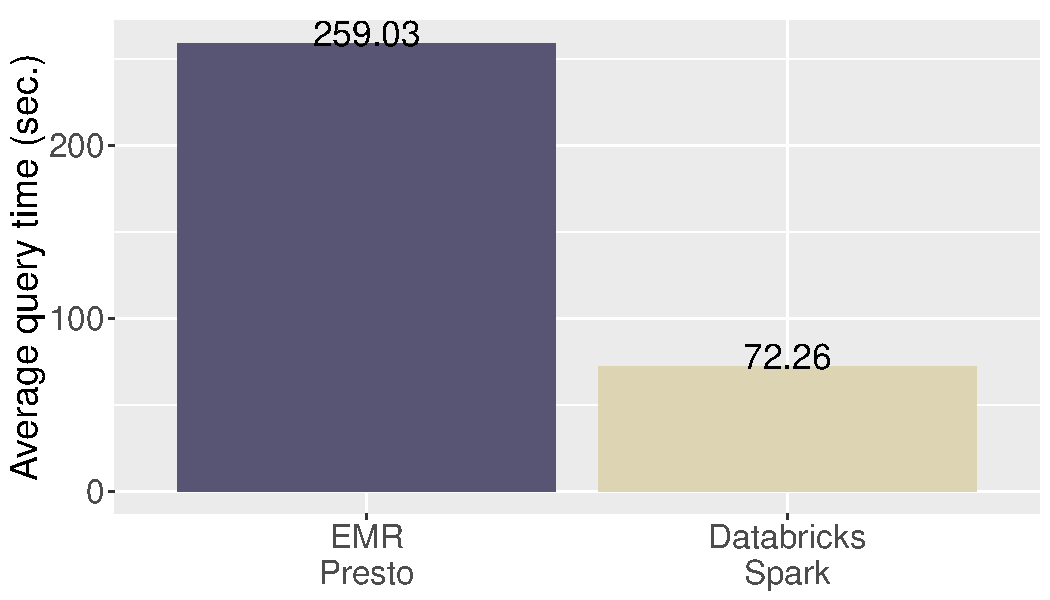
\includegraphics[width=7.0in]{imgs/referenceResults/power_avgTimeBarChart.pdf}}
   \end{center}
   \caption{Reference results Power Test query execution time arithmetic mean.}
   \label{fig:referenceResultsPowerTestArithmeticMean}
\end{figure}

The total execution time for the Power Test is roughly 2 hours for Databricks while it is over 7 hours for EMR Presto. The query execution time geometric mean and arithmetic mean for Databricks are also about 27\% of the corresponding metrics for EMR Presto. In addition to the aggregated metrics, we present a comparison of the execution time of individual queries in Figure \ref{fig:referenceResultsDataLoadingIndTimes1} to Figure \ref{fig:referenceResultsDataLoadingIndTimes5}.

\begin{figure}
   \begin{center}
   \scalebox{0.65}{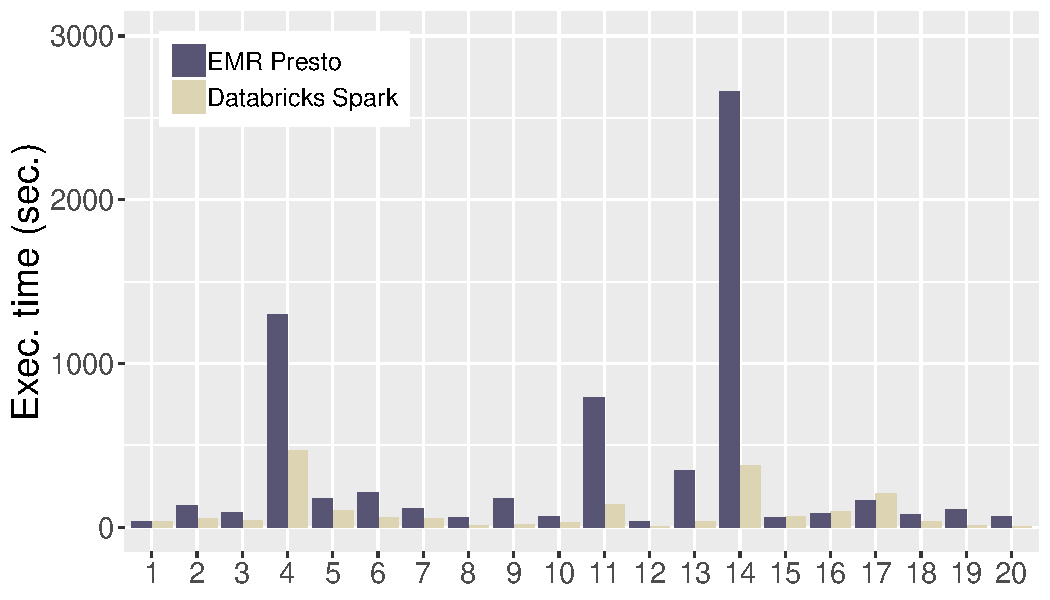
\includegraphics[width=7.0in]{imgs/referenceResults/powerTestIndivQueries1.pdf}}
   \end{center}
   \caption{Reference results Power Test individual query execution times (1).}
   \label{fig:referenceResultsDataLoadingIndTimes1}
\end{figure}

\begin{figure}
   \begin{center}
   \scalebox{0.65}{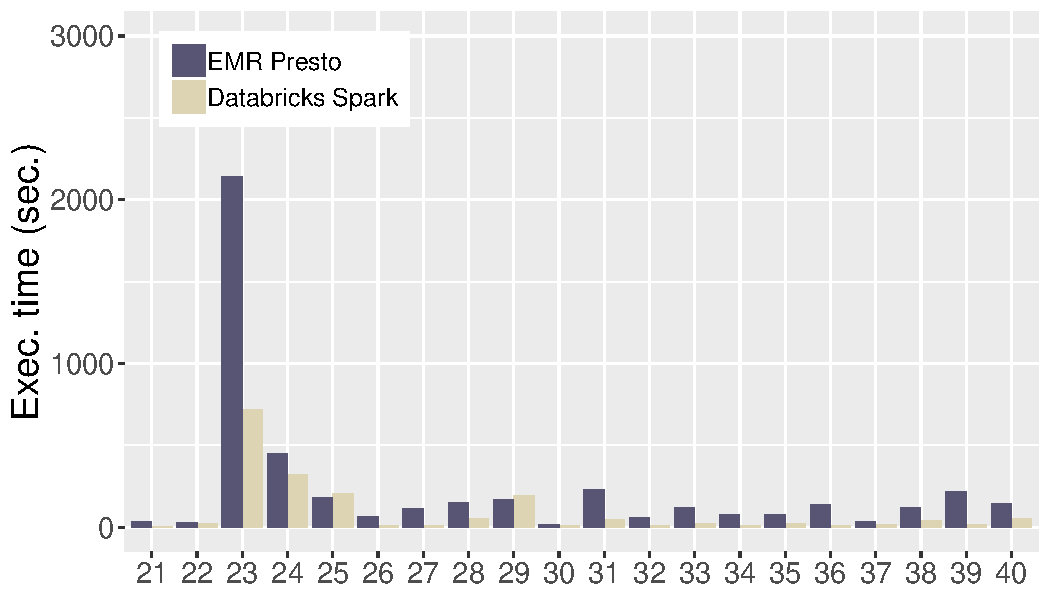
\includegraphics[width=7.0in]{imgs/referenceResults/powerTestIndivQueries2.pdf}}
   \end{center}
   \caption{Reference results Power Test individual query execution times (2).}
   \label{fig:referenceResultsDataLoadingIndTimes2}
\end{figure}

\begin{figure}
   \begin{center}
   \scalebox{0.65}{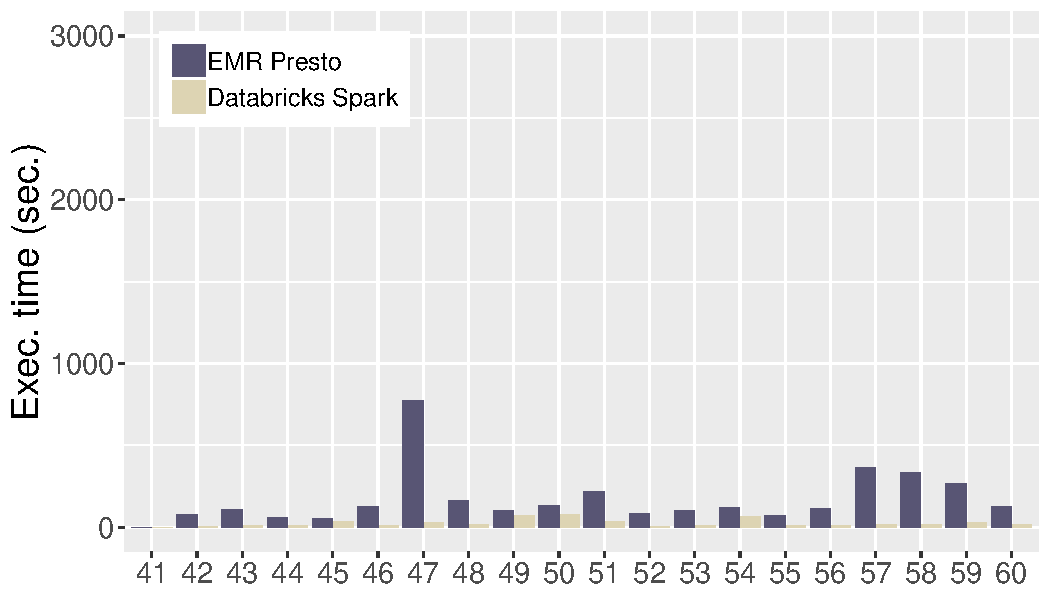
\includegraphics[width=7.0in]{imgs/referenceResults/powerTestIndivQueries3.pdf}}
   \end{center}
   \caption{Reference results Power Test individual query execution times (3).}
   \label{fig:referenceResultsDataLoadingIndTimes3}
\end{figure}

\begin{figure}
   \begin{center}
   \scalebox{0.65}{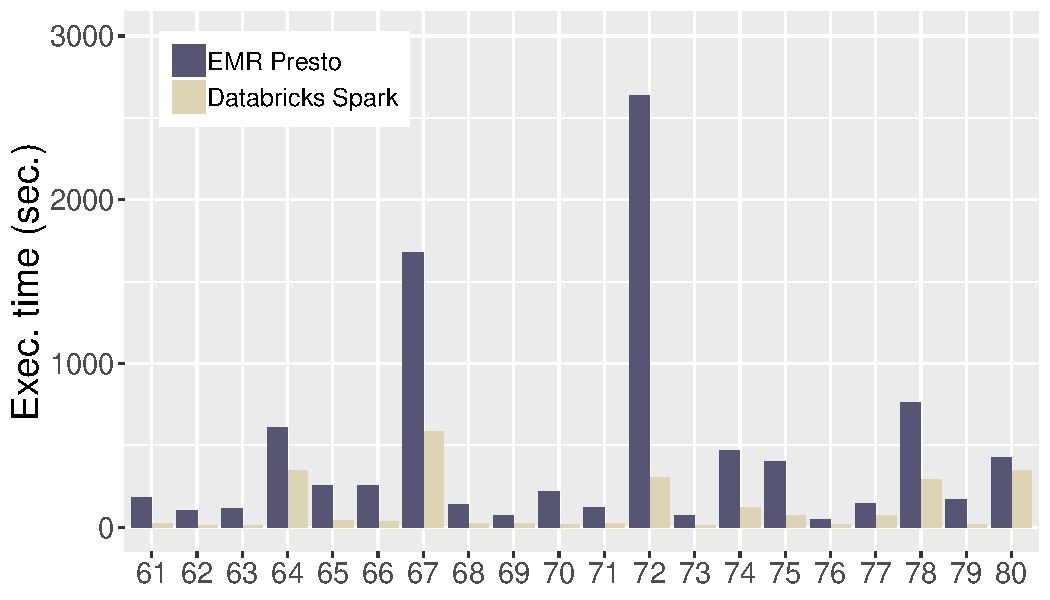
\includegraphics[width=7.0in]{imgs/referenceResults/powerTestIndivQueries4.pdf}}
   \end{center}
   \caption{Reference results Power Test individual query execution times (4).}
   \label{fig:referenceResultsDataLoadingIndTimes4}
\end{figure}

\begin{figure}
   \begin{center}
   \scalebox{0.65}{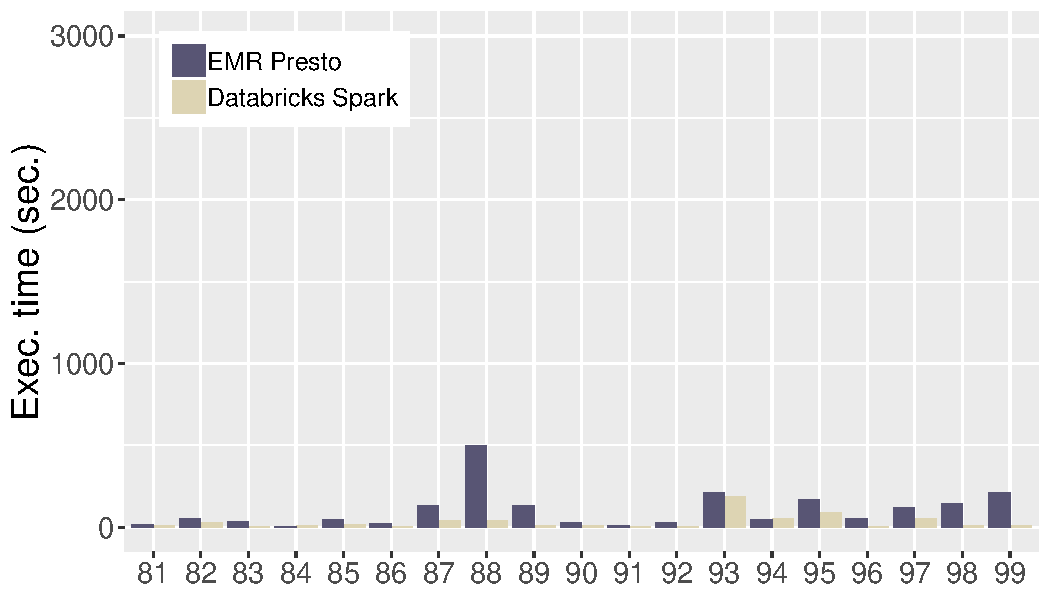
\includegraphics[width=7.0in]{imgs/referenceResults/powerTestIndivQueries5.pdf}}
   \end{center}
   \caption{Reference results Power Test individual query execution times (5).}
   \label{fig:referenceResultsDataLoadingIndTimes5}
\end{figure}

We must clarify that in the case of EMR Presto additional configuration parameters were specified through the benchmark execution code as session parameters applied to all queries unless they were overridden. We list these parameters in Listing \ref{listing:prestoConfigurationParameters}.

\vspace{0.5cm}

\begin{lstlisting}[caption={Reference results EMR Presto configuration parameters.},label=listing:prestoConfigurationParameters,captionpos=b,frame=single]
query_max_stage_count: 102
join_reordering_strategy: AUTOMATIC
join_distribution_type: AUTOMATIC
task_concurrency: 8

\end{lstlisting}

The maximum number of stages is set to 102 since that is the maximum generated among the 99 TPC-DS queries. The join reordering strategy and distribution type is set to automatic to enable the optimizer to select the best alternative. The task concurrency is set to 8, lower than the default 16, aiming to reduce global memory use. Some of these configuration parameters have to be overridden to enable the correct and efficient completion of some queries, Table \ref{table:prestoQueryConfigurationParameters} lists the queries involved and their settings.

\begin{table}
  \centering
	\begin{tabular}{|l|l|}
	  \hline
		\textbf{Queries} & \textbf{Configuration parameters} \\ \hline
		5, 75, 78, and 80 & join\_distribution\_type: PARTITIONED \\ \hline
		78 and 85 & join\_reordering\_strategy: NONE \\ \hline
		67 & task\_concurrency: 32
		\\
		\hline
	\end{tabular}
	\caption{Queries with specific configuration parameters for EMR Presto.}
	\label{table:prestoQueryConfigurationParameters}
\end{table}

The settings in Table \ref{table:prestoQueryConfigurationParameters} address the most common reason of failure, in our experience, for large scale queries in Presto, namely, exceeding the memory limit for a single node. Using distributed partitioned joins precludes this error for some queries. Disabling join re-ordering avoids generating excessively large intermediate results in some nodes for queries 78 and 85, albeit at probably slower execution times. The behavior of query 67 is harder to characterize, it would appear that possibly a large number of tasks prevents the system of trying to allocate blocks of memory that are too large for a single node to handle when computing the final aggregation.

In addition to the configuration parameters outlined above, queries 95 and 72 had to be modified to run successfully on EMR Presto while they ran satisfactorily in Databricks. In the case of query 95, unnecessary projected attributes were removed and a distinct clause was added to reduce the size of intermediate results. Even if this is known to be an expensive operation, it turned out to be an acceptable alternative to avoid the aforementioned memory error at a single node. As for query 72, joins were re-ordered manually, since the original order led to an extremely slow execution of more than 24 hours (in a test cluster with 4 worker nodes), while automatic re-ordering led to single node memory failures. The modified versions of queries 95 and 72 were employed for Databricks as well to obtain consistent results.

From the results depicted in Figure \ref{fig:referenceResultsDataLoadingIndTimes1} to Figure \ref{fig:referenceResultsDataLoadingIndTimes1}, we can observe that in most cases Databricks is more efficient that EMR Spark by a large margin, with queries 14, 23, and 72 being particularly slow on EMR Presto, taking more than 30 minutes. In a few cases, the completion time for EMR Presto was lower, concretely for queries 1, 15-17, 25, 29, 41, 84, and 94. However, in all cases it was by a small difference, the biggest difference being for query 17, which took 0.79 times the execution time in Databricks.

\subsection{Concurrent query execution (Throughput Test)}

The TPC-DS Throughput Test consists of running a certain number of query streams concurrently. A query stream implies running a permutation of the TPC-DS queries sequentially. The order of the query streams is given by the TPC-DS specification and results from randomization. For our reference results, we employ again the 1 TB scale factor and launch 4 query streams. Given that the TPC-DS benchmark includes 99 queries, the throughput test total is 396 queries. We present in Figure \ref{fig:referenceResultsTputTotalTime} the total execution time of the Throughput Test.

\begin{figure}
   \begin{center}
   \scalebox{0.65}{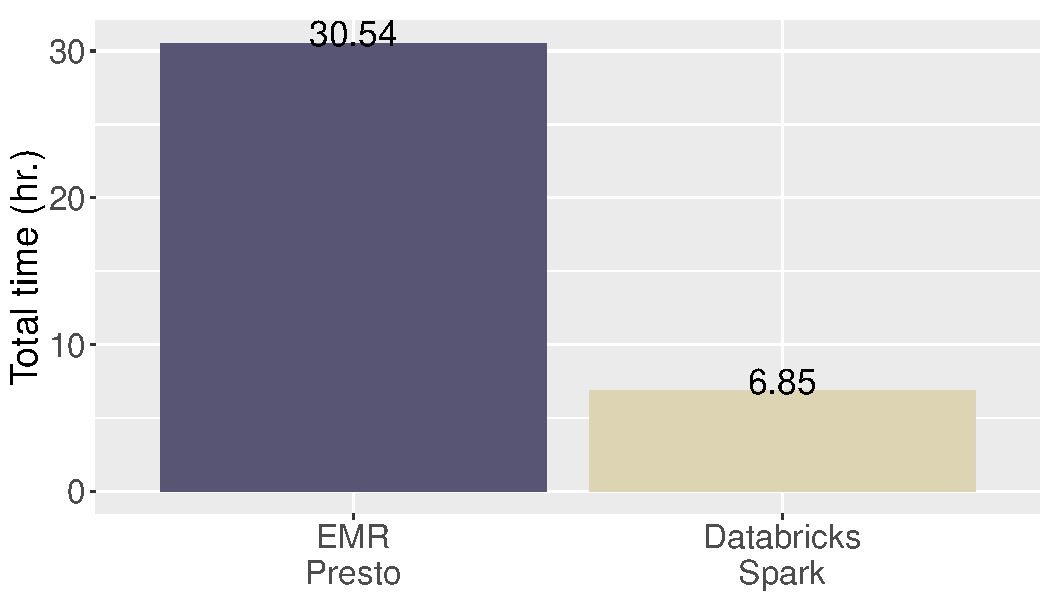
\includegraphics[width=7.0in]{imgs/referenceResults/tput_totalHrTimeBarChart.pdf}}
   \end{center}
   \caption{Reference results Throughput Test total time.}
   \label{fig:referenceResultsTputTotalTime}
\end{figure}

The total execution time for EMR Presto is over 30 hours, while it is less than 7 for Databricks. Recalling the Power Test execution times illustrated in Figure \ref{fig:referenceResultsPowerTestTotalTime}, we can determine that Databricks deals better with concurrency and thus makes a more efficient use of the available resources than EMR Presto. In fact, the purely sequential execution of all of the Throughput Test queries on Databricks would presumptively take 8.04 hours (4 times 2.01), while running the 4 concurrent streams measured 6.85 hours. EMR Presto, on the contrary, required 30.54 hours, higher than the estimate for sequential execution of 28.6 hours (4 times 7.15).

These results adhere to our observation that in many cases, EMR Presto executes for the most part only the tasks related to one of the queries, especially for memory intensive queries, while still having to deal with the overhead of concurrent queries. In extreme cases, there is essentially a single node completing a query while the other nodes are mostly idle.

\subsection{Benchmark costs}

We now present in Figure \ref{fig:referenceResultsTotalCosts} the monetary costs related to our reference results based on the pricing model described in Section \ref{systemPricing}. These total costs involve the Data Loading Test, the Power Test, and the 4-stream Throughput Test.

\begin{figure}
   \begin{center}
   \scalebox{0.65}{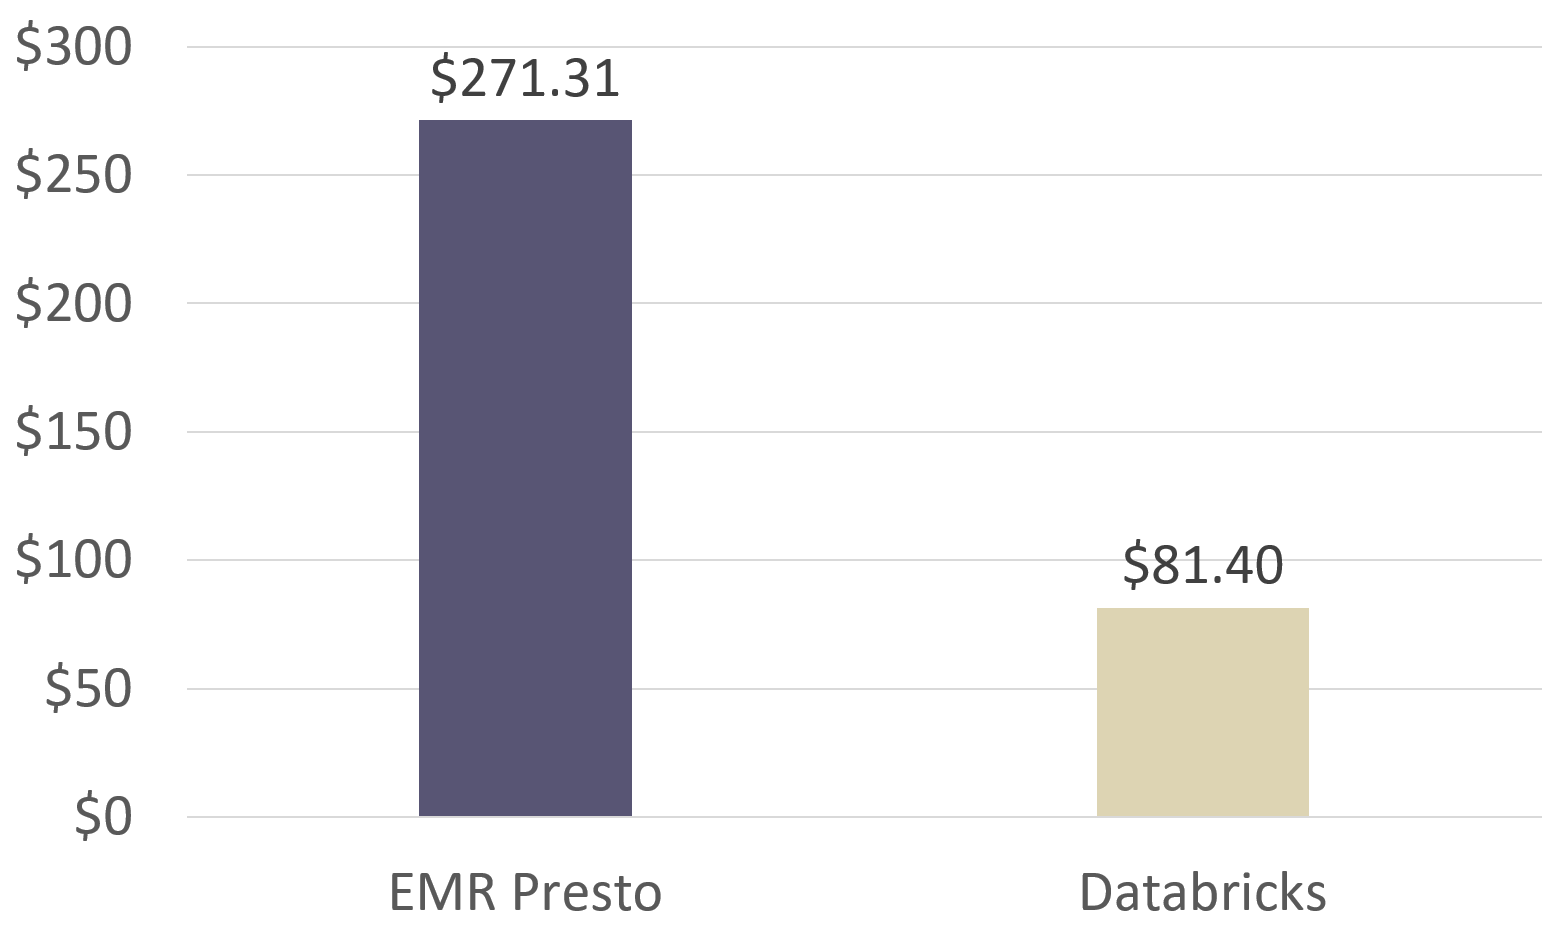
\includegraphics[width=7.0in]{imgs/referenceResults/ReferenceResultsCost.png}}
   \end{center}
   \caption{Reference results TPC-DS Benchmark total costs.}
   \label{fig:referenceResultsTotalCosts}
\end{figure}

The total cost of EMR Presto is more than 3 times that of Databricks (3.33 times to be precise). We can see that although the Databricks software price per hour per node is higher, its efficiency and resulting lower completion times matter the most for cost savings.



